\subsubsection{In Situ Process Monitoring and Feedback}
%\begin{figure*}
%	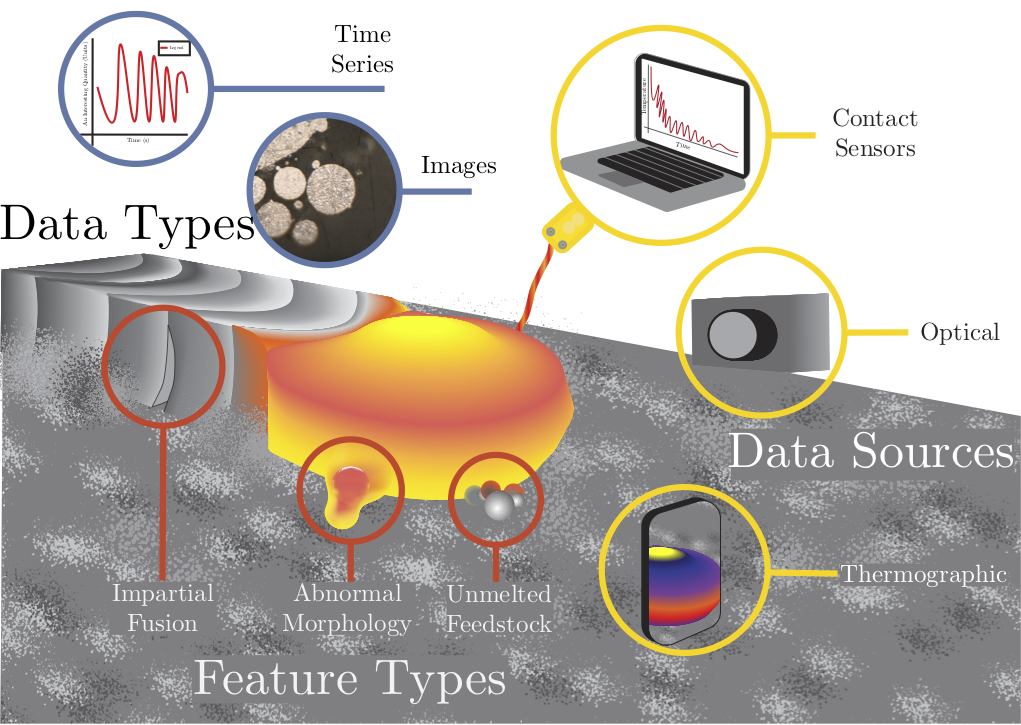
\includegraphics[width=0.85\linewidth]{Images/melt_pool}
%	\caption{}
%	\label{}
%\end{figure*}

\textbf{Need to include Kwon2018 \cite{Kwon2018} -- paper about using a NN for to classify melt-pool images}.

Thus far, in situ control in AM has been consistently ranked as one of the most-needed technologies for advancing the technology \cite{Berumen2010, Tapia2014, Mani2017}. The combination of rapid solidification and the small length scales of AM solidification can make traditional process monitoring approaches difficult. Machine learning can fill in gaps where human-specified process monitoring models are insufficient.

Computer vision can be employed in additive manufacturing to monitor the printing process, such as characterizing temperature profiles, identifying abnormal melt pool morphologies, and automatically detecting defect formation. Doing so will require methods for in situ process monitoring and data collection. 

Process monitoring involves acquisition of realtime signals which can reveal information about a wide variety of phenomenon during manufacturing. McKeown et al. used dynamic transmission electron microscopy to measure solidification rates in powder bed AM \cite{McKeown2016}. Bertoli et al. also characterized cooling rates using high speed imaging \cite{Bertoli2017}. Raplee et al. used thermography to monitor the solidification and cooling rates of electron beam powder bed fusion, then related the temperature profiles to defect and microstructural characteristics \cite{Raplee2017}. Distortion of parts due to thermal cycling was investigated by Denlinger et al. by means of thermocouples in contact with the build substrate \cite{Denlinger2015}. All of these methods are amenable to aid by computer vision and signal processing.

The type of data being collected in situ is most often in the form of time series data or images. Signal processing of either typically involves identifying signals which deviate from a mean, desired signal. Examples include a spike in temperature from a thermocouple or a sharp change in intensity in an image, both of which may indicate a deviation from the desired processing conditions. Image processing tools known as \textit{filters} can be used to identify signals of interest in AM data. From a mathematical perspective, filters are implemented for signal/image processing in the same way as for topology optimization. 

A filter is implemented as mathematical operation on a segment of time series data or an area of pixels in an image. The simplest filters identify characteristics of the pixel intensity in that region and highlight them. An example for an image would be to identify regions of sharp change in intensity, which often correspond to boundaries between objects. An example would be the change in intensity between a liquid melt pool and the powder bed. Signals of interest or regions of interest in an image identified by filters are known as \textit{features}. 

The use of filters alone does not constitute machine learning, but filters can be used in regression algorithms to learn signal features which are indicative of behavior in the manufacturing process. Defect detection is an apt use of filters in a machine learning approach. Repeated defect-free printing involves following the same processing parameters every manufacture. Regression algorithms can predict when a defect appears by monitoring when features indicative of defects are found by filters. 

A computer vision method called  \textit{template matching} can be utilized for automatic identification of signal features. Template matching involves comparison of a database of pre-identified signal features with the features measured in situ. The scale-invariant feature transform (SIFT) \cite{Lowe2004} and a variant of it, speeded-up robust features (SURF) \cite{Bay2008} are both feature identification algorithms which can be used for template matching. A specific type of template matching is the `bag of visual words' or `dictionary' method. A collection (dictionary) of typical features from the AM process can be built based on features obtained from filters. The features measured in situ are compared with dictionary entries. If an in situ feature matches a defect-indicative feature from the dictionary, then it is likely a defect has formed in manufacturing process. 

Template matching is carried out through similarity of analysis of in situ features and dictionary features. Outputs of filters can also be used as inputs to regression algorithms to predict the probability of a feature being present in an image. For example, an algorithm may be trained which convolves three different filters with a signal acquired in situ. Each filter likely highlights a different aspect of the signal. The goal of the algorithm is to predict whether or not a defect is present in pixel location $P(x,y)$. A regression algorithm can be trained
\eqn
	P(x,y) = w_1 I_1(x,y) + w_2 I_2(x,y) + w_3 I_3(x,y)
	\label{filterregress}
\equ
where the probability of a defect being present is dependent upon the results of filter operations on regions of the image. This type of algorithm is the basis for a \textit{neural network} where filters are used as regression functions for feature identification in images. Recently, advances in computer vision has led to the advent of \textit{convolutional neural networks} which have high prediction accuracy for feature identification in images. 

Convolutional neural networks not only adjust the weights $w_i$ of regression algorithms for feature identification, but also adjust the filters themselves. That is, convolutional neural networks `learn' the best filters for elucidating features which are indicative of process phenomenon.  CNNs use large databases of labeled information to learn features in the image that indicate whether or not certain human-identified objects are present. Convolutional neural networks can identify multiple features or defects in an image simultaneously. A downside to CNNs is that they require \textbf{very} large datasets (thousands of images, at the least) of labeled data to be successful. Neural networks have already been implemented for in situ AM analysis. Yuan et al \cite{Yuan2018} were able to successfully monitor melt track width, standard deviation, and continuity of tracks in situ during laser powder bed manufacturing. Scime and Beuth trained a convolutional neural network to identify six different types of defect which are typical of laser powder bed fusion, with fairly good prediction accuracy \cite{Scime2018}. These studies encompass only a few of the possibilities of in situ process monitoring for AM. 



